\documentclass[10pt,a4paper]{article}
\usepackage[utf8]{inputenc}


\usepackage[T1]{fontenc}
\usepackage{fontspec}

% Spécifiez ici la police que vous souhaitez utiliser
\setmainfont{Times New Roman }

\usepackage{amsmath}
\usepackage{amsfonts}
\usepackage{amssymb}
\usepackage{graphicx}
\usepackage{mdframed}

\usepackage{pgfplots}
\pgfplotsset{compat=1.18}
\usepackage{lmodern}
%\usepackage{kpfonts}
\usepackage{circuitikz}
\usepackage[left=2cm,right=2cm,top=2cm,bottom=2cm]{geometry}
\usepackage[most]{tcolorbox}
\tcbset{sabour/.style={enhanced,title=EXERCICE 1, coltitle= black,colbacktitle= blue!20,colback=white,fonttitle=\bfseries,
boxed title style={colback=blue!25}}}
\usepackage{fancyhdr}

\pagestyle{fancy}

\fancyhf{}

\lhead {Mr SABOUR}
\chead{LES LOIS DE NEWTON }
\rhead {2ème Bac SM}
\lfoot{fiches de Mr SABOUR pour $2\textsuperscript{ème}$ AC  SM  : Mécanique}

\rfoot{Page \thepage}
\renewcommand{\footrulewidth}{0.05pt}

\begin{document}


 Pour tous les exercices prendre $g = 10m.s^{-2}$
\begin{tcolorbox}[sabour]
L'équation horaire du mouvement d'un mobile M sur un axe $(OX)$ est $ x=4t^2-2t +5$.
\begin{enumerate}
\item Trouver les expressions de vitesse $v(t)$ et de son accélération $a(t)$.
\item à quelle date $t_1$  et en quel point $M_1$  le mouvement change de sens ?
\item Quelle est la nature du mouvement du point M? accélérée retardé.... et sur quel intervalle ?)
\item Déterminer la date du passage du mobile par le point de départ? quelle est alors la valeur de sa vitesse?
\item Quelle distance parcourt-t-il quand sa vitesse passe de $V_1=-1m/s $ à  
$V_2=1m/s$.
\end{enumerate}

\end{tcolorbox}

\begin{tcolorbox}[sabour,title=EXERCICE 2]
Au moment où le bus démarre sur une voie rectiligne à l'accélération de $a=2m.s^{-2}$, Driss qui se trouve à $d_0= 10m $ derrière décide de courir à la vitesse constante de $V=6m/s$. rattrapera -t-il son bus? sinon quelle set la distance minimale qui le sépare de son bus?

\end{tcolorbox}

\begin{tcolorbox}[sabour,title=EXERCICE 3]
\begin{minipage}{9cm}
Un mobile part de l'origine d'espace à la date $t=0 s$ où il se meut sur une trajectoire rectiligne (OX)

\begin{enumerate}
\item Déterminer graphiquement l'accélération du mouvement
\item En déduire  l'équation horaire de la vitesse 
\item Trouver la date de changement de sens du mouvement 
\item Quelle est la nature du mouvement
\item Écrire l'équation horaire de la position . Quel est la position du point de changement de sens du mouvement?
\item Calculer la distance parcourue par le mobile entre les instants $t=0s $ et $t_2=1,5s$.
\end{enumerate}
\end{minipage}
\begin{minipage}{8cm}


    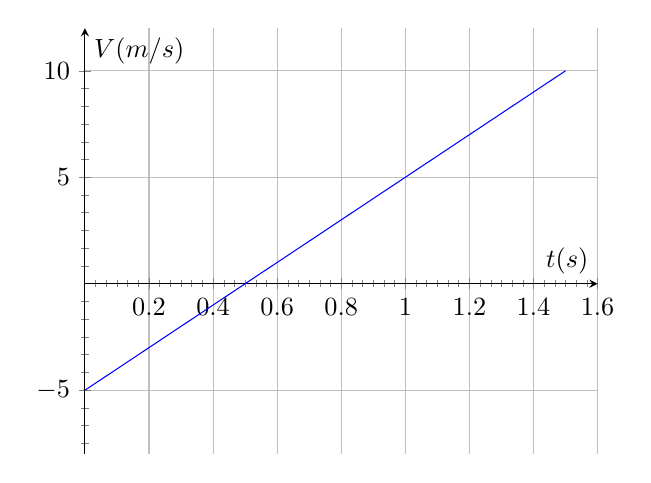
\begin{tikzpicture}[scale=0.95]
        \begin{axis}[
            xlabel={$t(s)$},
            ylabel={$V( m/s)$},
            axis lines=middle,
            xmin=0, xmax=1.6,
            ymin=-8, ymax=12,
            domain=0:1.5,
            samples=100,
            grid, % Activer la grille
            minor tick num=5, % Nombre de divisions mineures entre chaque marqueur majeur
        ]
            \addplot[blue] {10*x -5)};
        \end{axis}
    \end{tikzpicture}
\end{minipage}
\end{tcolorbox}

\begin{tcolorbox}[sabour,title=EXERCICE 4]
un bus part de l'origine du repère (O,X) sur une voie rectiligne avec une accélération constante  $a_1=0,5m.s^{-2}m/s$ et quand il atteint le point A il lève le pied pour que son mouvement soit rectiligne uniforme pendant $1min$ arrivé au point B il freine avec une accélération constante $a'=-2m.s^{-2}$ et il s'arrête au point C parcourant la distance totale$ OC=500m$.
\begin{enumerate}
\item La vitesse du point A 
\item La durée du mouvement accéléré et la distance $OA$
\item Calculer la vitesse moyenne le long du trajet $OC$ ?
\end{enumerate}
\end{tcolorbox}
\begin{tcolorbox}[sabour,title=EXERCICE 5]
l'équation horaire d'un M.R.U.V est $x=\frac{1}{2}at^2$
montrer que les espaces parcourus pendant des intervalles de temps succéssifs égaux à $\tau = 40ms $ forment une suite arithmétique 
de raison $r=a.\tau^2$ calculer a sachant que la raison est $r=5,88\times10^{-3}m$ .



\end{tcolorbox}

\begin{tcolorbox}[sabour,title=EXERCICE 6]
Un automobiliste se déplace à la vitesse de $V_i = 16m/s$  au moment où le feu vert qui se trouve en face de lui à la distance $D=200m$ s'allume, il reste allumé pendant $11s$. Cet instant sera pris comme origine du temps $t=0s$ , et la position de la voiture à cette date comme origine de l'axe  du mouvement (OX).
L'automobiliste impose à sa voiture une accélération constante  pendant une durée $t_1$ ,  sa vitesse passe à  $V_1=21m/s$ après un parcourt de $x_1=100m$.

\begin{enumerate}
\item Déterminer 
\begin{enumerate}
\item[1.1)] L'accélération $a_1$ 
\item[1.2)] La date $t_1$ 
\item[1.3)] Écrire l'équation horaire de la position $x(t)$.
\end{enumerate}
\item jugeant qu'il peu passer , l'automobiliste maintient sa vitesse constante $V_1$ à partir de la date $t_1$
\begin{enumerate}
\item[2.1)] Écrire l'équation horaire du mouvement après la date $t_1$.
\item[2.1)] La voiture passera-t-elle devant le feu quant il est vert?
\end{enumerate}
\item Le chauffeur  juge qu'il ne peut pas passer, à la date $t_1$ il freine d'un mouvement uniformément retardé d'accélération $a_2 =-2m/s^2$.
\begin{enumerate}


\item[3.1)] Calculer la distance parcourue par la voiture pendant le freinage jusqu'à l'arrêt complet
\item[3.1)] à quel instant $t_2$ et avec quelle vitesse $v_2$ la voiture passe devant le feu rouge?
\end{enumerate}
\end{enumerate}

\includegraphics[scale=0.5]{voiture _feu_rouge.png} 



\end{tcolorbox}

\begin{tcolorbox}[sabour,title=EXERCICE 7]
Les équations horaire du mouvement d'un mobile dans le repère $(O,X,Y) $ est donnée par 
$$\vec{OM}=
(2t-2) \vec{i}+(-2t^2 + 4t)\vec{j}$$
\begin{enumerate}
\item  Exprimer les vecteur vitesse $\vec{V}$ et accélération $\vec{a}$. et en déduire leurs expressions en fonction du temps .
\item Quelle est la nature du mouvement sur chaque axe
\item Trouver l'équation de la trajectoire , quelle est sa nature .
\item soit $(S)$ le sommet de la trajectoire. Trouver ses coordonnées et montrer qu'en ce point $\vec{v}\times\vec{a}=0$ 
\item on considère la date $t_1=2 s$ 
\begin{enumerate}
\item[4.1)] Trouver les coordonnées de la position $M_1$ du mobile à cette date
\item[4.2)] Représenter le vecteur vitesse $V_1$
\item[4.3)] Tracer le repère de Frenet 
\item[4.3)] Tracer le vecteur accélération à la date $t_1$.
\item[4.4)] Tracer les composantes $a_T$ et $a_N$ du vecteur accélération $\vec{a}$ dans la base de Frenet et déterminer graphiquement leur valeurs 

\end{enumerate}
\end{enumerate}
\end{tcolorbox}


\begin{tcolorbox}[sabour,title=EXERCICE 8]
Les équations horaire du mouvement d'un mobile dans le repère $(O,X,Y) $ est donnée par 
$$\vec{OM}=
2t \vec{i}+(-5t^2 + 6t)\vec{j}$$
\begin{enumerate}


\item Trouver l'équation de la trajectoire , quelle est sa nature .
\item  Exprimer les vecteur vitesse $\vec{V}$ et accélération $\vec{a}$. et en déduire leurs expressions en fonction du temps .
\item (pour SM) 
\begin{enumerate}
\item[3.1)]Déterminer l'expression de l'accélération tangentielle $a_T$  en fonction du temps .
\item[3.2)] Déterminer l'expression de l'accélération normale $a_N$ en fonction du temps .
\item[3.3)] En déduire l'expression du rayon de courbure $\rho$ en fonction du temps . Calculer sa valeur à la date $t=1s$.
\end{enumerate}
\end{enumerate}
\end{tcolorbox}

\begin{tcolorbox}[sabour,title=EXERCICE 9]

Un point matériel est lancé de l'origine d'un repère $R(0,X,Y)$ avec une vitesse $\vec{V_0}$ qui fait l'angle $\alpha$ avec l'horizontale $(0X)$ .  par 
pointage et en utilisant un mlogiciel approprié on a pu tracer les courbes qui représentent les variations les composantes du vecteur vitesse $V_X$ et $V_Y$ en fonction du temps comme le montre la figure ci-contre.


\begin{minipage}{10cm}
\begin{enumerate}
\item Trouver graphiquement les équations horaires $V_X(t)$ et $V_Y(t)$.
\item Calculer la valeur de la vitesse initiale $\Vert\vec{V_0}\Vert$ ainsi que la valeur de l'angle $\alpha$.
\item En déduire les coordonnées du vecteur accélération
\item Quelle est la nature du mouvement sur chaque axe 
\item trouver les équations horaires du mobile dans le repère $R(0,X,Y)$ $x(t)$ et $y(t)$.
\item Trouver l'équation de la trajectoire. Quelle est sa nature ?
\item Calculer l'angle que fait l'accélération avec la normale dans la base de Frenet aux dates $t_1=1s$ et $t_2=1,5s$.
\end{enumerate} 
\end{minipage}
\begin{minipage}{8cm}





  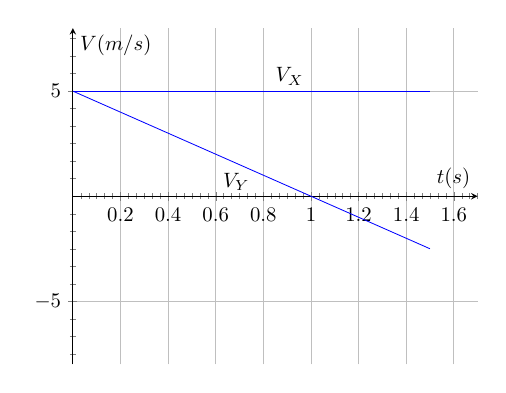
\begin{tikzpicture}[scale=0.75]
        \begin{axis}[
            xlabel={$t(s)$},
            ylabel={$V( m/s)$},
            axis lines=middle,
            xmin=0, xmax=1.7,
            ymin=-8, ymax=8,
            domain=0:1.5,
            samples=100,
            grid, % Activer la grille
            minor tick num=5, % Nombre de divisions mineures entre chaque marqueur majeur
        ]
            \addplot[blue] {-5*x +5)};
             \addplot[blue] {5)};
               \node[left] at (1,5.7) {$V_X$};
                 \node[right] at (0.6,0.7) {$V_Y$};
        \end{axis}
    \end{tikzpicture}


\end{minipage}
\end{tcolorbox}



\begin{tcolorbox}[sabour,title=EXERCICE 10]

Un corps ponctuel tombe en chute libre à partir d'un point O, origine du repère $(OZ)$ orienté vers le bas, où il part sans vitesse initiale à la date $t=0s$ 
\begin{enumerate}
\item Définir la chute libre 
\item appliquer la deuxième loi de Newton pour trouver l'accélération a du mouvement. 
\item Quelle est la nature du mouvement ? 
\item Écrire les équation horaires de la vitesse v(t) et de la position z(t)
\item Calculer la vitesse $V_1$ du mobile et trouver son abscisse $z_1$ à la date $t_1=2 s$
\end{enumerate}

\end{tcolorbox}
\begin{tcolorbox}[sabour,title=EXERCICE 11]
Du même point on lance vers  verticalement vers le haut deux billes;  la bille A d'abords à la date $t=0s$ et la bille B après une seconde. les deux billes ont la même vitesse initiale $V_0=10m/s$ et sont considérés en chute libre  . quand et où? vont elle se rencontrer?

\end{tcolorbox}


\begin{tcolorbox}[sabour,title=EXERCICE 12]
Une bille abandonnée sans vitesse initiale parcourt le dixième de sa hauteur totale $\frac{h}{10} $  dans sa dernière seconde de chute 
\begin{enumerate}
\item Calculer la durée de chute et la hauteur parcourue pendant la dernière seconde 
\item Calculer la vitesse d'arrivée au sol 
\end{enumerate}
\end{tcolorbox}

\begin{tcolorbox}[sabour,title=EXERCICE 13]
Un projectile est lancé verticalement de la surface du sol. Un système de détection enclenche un chronomètre  l'instant de départ et enregistre les dates$ t_1$ et $t_2$  de passage du projectile dans le plan horizontal d'altitude h.
\begin{enumerate}

\item  A quelle date et avec quelle vitesse le projectile retombe-t-il sur le sol ? 
\item Déterminer la vitesse de lancement et l'altitude h en fonction des dates $t_1$ et $t_2$. 
A.N : $t_1 = 0,875s$ , $ t_2 = 9,329s$ .

\end{enumerate}
\end{tcolorbox}


\begin{tcolorbox}[sabour,title=EXERCICE 14]


 Une caisse (C) glisse sans frottement le long d'un plan incliné depuis le point O vers le point A loin de $x_A=10m$ en bas . voir figure 
 \begin{enumerate}
 \item  Reproduire le schémas sur votre copie et représenter sans échelle les forces qui agissent sur (C).
 \item Déterminer  les coordonnées du poids$ \vec{P}$ et en fonction de m, g et $\alpha$ et celle du vecteur $ \vec{R}$ , dans le repère $(0,X,Y) $ .
 \item appliquer la deuxième loi de Newton pour trouver l'accélération a du mouvement. Quelle est la nature du mouvement ? 
 \item  Sachant que l'accélération $a=5m/s^2$ calculer la valeur de l'angle $\alpha$
 \item Écrire v(t) et x(t). 
 \item Calculer la date de passage par le point A. Quelle est la valeur de la vitesse $V_A$  en A .
 \item On refait l'expérience en lançant le corps (C)  , sur le plan incliné , vers le haut à la vitesse $V_0=6m/s$ . 
\begin{enumerate}
\item[7.1)] L'accélération du mobile change -t-elle?
\item[7.2)] écrire les nouvelle expressions de la vitesse v(t) et de la position x(t) 
\item[7.3)]  A quelle date le mouvement du mobile change de sens ? quelle est alors sa position 
\item[7.4)] à quelle date le mobile passe par O de nouveau?
\item[7.5)] Calculer la vitesse de passage du mobile par le point A.
\end{enumerate}
 \end{enumerate}
\begin{center}
\includegraphics[scale=0.7]{mvt sur plan incliné.png} 
\end{center}

\end{tcolorbox}
\begin{tcolorbox}[sabour,title=EXERCICE 15]
\begin{minipage}{10cm}
Sur un plan incliné d'un angle $\alpha $ par rapport à l'horizontale , on lance vers le haut un solide (S) ponctuel.
Le diagramme des vitesse d'un mobile sur une voie rectiligne est représenté sur la figure ci-contre 
\begin{enumerate}
\item Déterminer l'équation horaire de la vitesse 
\item le mouvement change de sens au point H ? calculer$t_H$
\item le mobile passe par l'origine des espaces à la date $t=2s$  Trouver la position $x_0$ du mobile à la date $t=0s$ . et trouver la position $x_H$ du point H
\end{enumerate}
\end{minipage}
\begin{minipage}{8cm}
    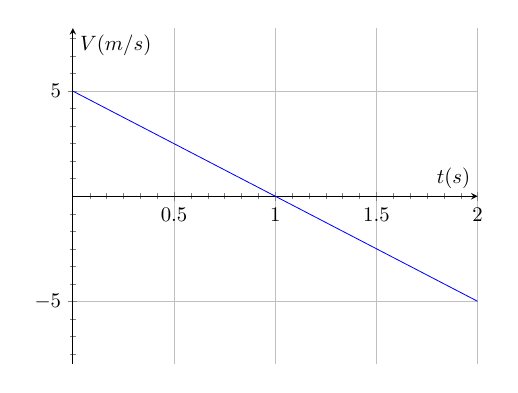
\begin{tikzpicture}[scale=0.75]
        \begin{axis}[
            xlabel={$t(s)$},
            ylabel={$V( m/s)$},
            axis lines=middle,
            xmin=0, xmax=2,
            ymin=-8, ymax=8,
            domain=0:2,
            samples=100,
            grid, % Activer la grille
            minor tick num=5, % Nombre de divisions mineures entre chaque marqueur majeur
        ]
            \addplot[blue] {-5*x +5)};
            
        \end{axis}
    \end{tikzpicture}
\end{minipage}


\end{tcolorbox}


\begin{tcolorbox}[sabour,title=EXERCICE 16]

un solide (C) glisse avec le long d'un plan incliné d'un angle $\theta$=30\.° avec l'horizontale , depuis le point O vers le point A loin de $x_A=10m$ en bas . voir figure . on note $ k=\tan \varphi$  le coefficient de frottement  et $\varphi$ l'angle de frottement 
 \begin{enumerate}
 \item  Reproduire le schémas sur votre copie et représenter sans échelle les forces qui agissent sur (C).

 \item En  appliquant  la deuxième loi de Newton montrer que l'expression de  l'accélération a du mouvement est donnée par : 
 $$ a= g (sin\theta - kcos\theta)$$ . Quelle est la nature du mouvement ? 

 \item Écrire v(t) et x(t). 
  \item  la vitesse de passage par le point A est $V_A=8m/s$ , calculer l'accélération a   
\item En déduire la valeur du coefficient de frottement k et la valeur de l'angle de frottement.

\end{enumerate}
\begin{center}
\includegraphics[scale=1]{plan incliné coloré.png} 
\end{center}
\end{tcolorbox}
\begin{tcolorbox}[sabour,title=EXERCICE 17]

On lance vers le haut un solide ponctuelle sur un plan inclnée de l'angle $\alpha=$30° à la vitesse $\vec{V_0}$ de l'origine du repère (O,X,Y). il repasse par le point A située la distance d plus bas à la vitesse $\vec{V_A}= - \vec{V_0} $. sachant que le coefficient de frottement $K=0,2$ est le même pendant la montée et pendant la descente , calculer $V_0$, la durée du mouvement ainsi que la vitesse moyenne du parcourt. Prendre $g=10m.s^{-2}$
\end{tcolorbox}


\begin{tcolorbox}[sabour,title=EXERCICE 18]

On considère un véhicule de masse $m = 1000K $ en mouvement sur une piste inclinée d'un angle $\alpha = $30° par rapport au plan horizontal.

 Au cours de son mouvement, le véhicule est constamment soumis à des forces de frottement dont la résultante $\vec{f} $ est dirigée dans le sens contraire au vecteur vitesse et a pour valeur $f =400N$.
 
Lorsque le véhicule se déplace, son centre d'inertie G décrit la ligne de plus grande pente représenté par l'axe $XX'$ 

\begin{enumerate}


\item  Sous l'effet d'une force motrice $\vec{F}$ F, développée par le moteur et de même direction que la ligne de plus grande pente, le véhicule quitte la position A avec une vitesse nulle et atteint la position B avec une vitesse de valeur $V_B=20m/s$1. La distance entre A et B est  $AB = 10m$. Montrer que l'expression de la force motrice est :

$$  F= mg\sin \alpha +f +\dfrac{m.v_B^2}{2.AB}$$
Calculer F
\item  Lorsque le véhicule passe en B, la force F est supprimée. Le véhicule continue son mouvement jusqu'à la position C où sa vitesse s'annule. Monter que: 
$$ BC = \dfrac{mV_B^2}{2(f+mg\sin \alpha)}$$
Calculer BC.
\item Quelle doit être la nouvelle valeur de F pour que le véhicule atteint le point D avec une vitesse nulle.
On donne BD =AB.

\end{enumerate}

\begin{center}

\includegraphics[scale=1]{mvt ascendant plan incliné.png} 

\end{center}


\end{tcolorbox}


\begin{tcolorbox}[sabour,title=EXERCICE 19]
Sur un plan inclinée d'un angle $\alpha= $30°  par rapport à l'horizontale ,on lance une solide ponctuel de masse $m=400g$  vers le haut avec une vitesse  $ \vec{V_0}$. soit $k$ le coefficient de frottement  
l'étude est faite dans une référentielle terrestre supposé Galiléen au quel on associe le repère (O,X,Y): (OX) étant confondu avec la ligne du plus grande pente du plan incliné orienté vers le haut  
Le corps est considérée  en chute libre.

 La courbe ci-contre représente le diagramme des espaces $x=f(t)$ et la tangente à cette courbe à la date $t=0s$

\begin{enumerate}
\item Appliquer la deuxième lois de newton pour  trouver l'expression de l'accélération du mobile 
\item Déterminer la vitesse initiale? 
\item à quelle date le mouvement change de sens ?
\item En déduire l'accélération  du mouvement 
\item Calculer alors , l'intensité f de la force de frottement $\vec{f}$ et  le coefficient de frottement  $k$
\item Montrer que l'expression de l'intensité R' de la force $\vec{R'}$ exercée par le solide sur le plan inclinée est donnée est : $R'=f\sqrt{1+\frac{1}{k^2}}$ et Calculer sa valeur 
\end{enumerate}

  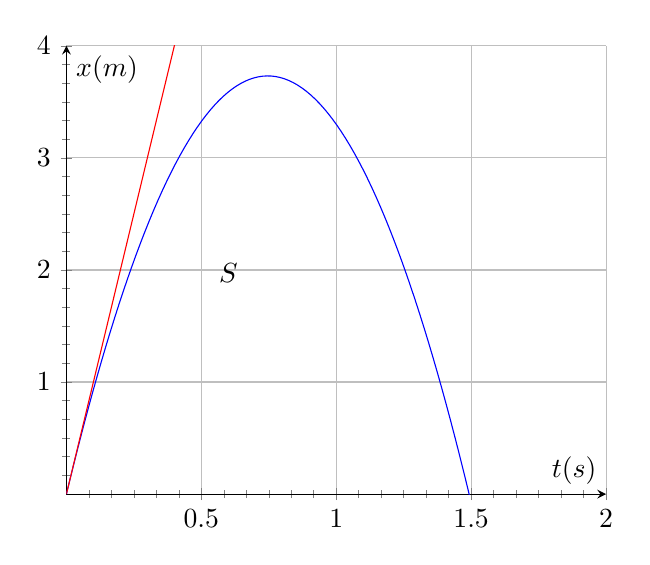
\begin{tikzpicture}[scale=1]
        \begin{axis}[
            xlabel={$t(s)$},
            ylabel={$x( m)$},
            axis lines=middle,
            xmin=0, xmax=2,
            ymin=0, ymax=4,
            domain=0:1.6,
            samples=100,
            grid, % Activer la grille
            minor tick num=5, % Nombre de divisions mineures entre chaque marqueur majeur
        ]
            \addplot[blue] {-6.7*x^2 +10*x)};
             \addplot[red] {10*x};
          %   \addplot[red] {1.8};
             %  \node[left] at (0,0.1) {$ X_m$};
                \node[above] at (0.6,1.8) {$S$};
        \end{axis}
    \end{tikzpicture}
\end{tcolorbox}

\begin{tcolorbox}[sabour,title=EXERCICE 20]
\begin{minipage}{11cm}
Un point matériel (S) est astreint à se mouvoir sans frottement sur un quart d'une sphère de rayon r. il part du sommet A avec une vitesse initiale négligeable. Déterminer la position où (S) quitte la sphère. \\


Indication : 
\begin{itemize}
\item Trouver l'expression de la vitesse en M par une méthode de votre choix ( théorème de l'énergie cinétique ou conservation de l'énergie mécanique)
\item Au point où (S) quitte la trajectoire  il n'y a plus de réaction $\vec{R}$ 
\end{itemize}
\end{minipage}
\begin{minipage}{8cm}
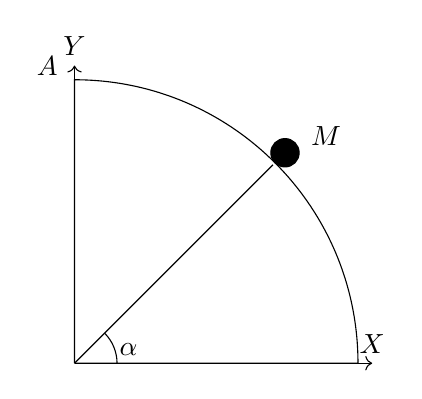
\begin{tikzpicture}[scale=0.9]
  % Définition des paramètres
  \def\r{4cm} % rayon du cercle
  \def\a{0} % angle de début du quart de cercle
  \def\b{90} % angle de fin du quart de cercle\\
 
  
  % Dessin du quart de cercle
  \draw (0,0) -- (\a:\r) arc (\a:\b:\r) -- (0,0);
  \draw (0,0) -- (2.8,2.8);
  % Dessin du corps ponctuel
  \filldraw (\a+45:\r+0.2cm) circle (0.2cm);
   % Dessin de l'angle alpha
  \draw (0.6,0) arc (0:45:0.6);
  \node[right] at (0.5,0.2) {$\alpha$};
   \node[left] at (-0.1,4.2) {$A$};
   \node[right] at (3.2,3.2) {$M$};
   \draw [->](0,0) to(4.2,0) node[above]{$X$};
 \draw [->](0,0) to(0,4.2) node[above]{$Y$};
\end{tikzpicture}
\end{minipage}

\end{tcolorbox}





\begin{tcolorbox}[sabour,title=EXERCICE 21]

Une petite sphère S, de rayon négligeable, de masse$ m = 200g$ est accrochée à un fil de masse négligeable, inextensible, de longueur $ l = 1m$. L'autre extrémité du fil est attachée  un point fixe. 

On écarte S de sa position d'équilibre verticale. Le fil tendu fait un angle 
$\theta_m $ avec la verticale. On lâche la sphère sans vitesse initiale.

\begin{minipage}{11cm}


\begin{enumerate}

\item Donner l'expression de la vitesse de S en fonction de l’angle que fait le fil avec la 
verticale. Calculer cette vitesse au passage à la position verticale. 
\item Exprimer l’accélération normale en fonction de $\theta$. Calculer sa valeur pour $\theta$= 0°.
\item Donner l'expression de la valeur de la tension du fil en fonction de $\theta$ . Calculer sa valeur maximale.
\item Exprimer l'accélération tangentielle en fonction de $\theta$ . Vérifier qu'elle s'annule lorsque la valeur de la tension est maximale 
\end{enumerate}
\end{minipage}
\begin{minipage}{6cm}
\includegraphics[scale=1.8]{tension T d'un pendule.png} 

\end{minipage}


\end{tcolorbox}

\begin{tcolorbox}[sabour,title=EXERCICE 22]

\begin{minipage}{11cm}
Une bille assimilable  un corps ponctuel peut glisser sans frottement à l'intérieur d'un cerceau vertical, de rayon r et de centre O. 

\begin{enumerate}
\item Exprimer l'intensité R de la réaction du cerceau en fonction de $V_0$, de g, de r et de m(masse de la bille) lorsque la bille est au point B diamétralement opposé à A. 
\item En déduire la valeur minimale de $V_0$ pour que la bille reste en contact avec la gouttière durant toute trajectoire circulaire. 
\end{enumerate}

\end{minipage}
\begin{minipage}{8cm}
\includegraphics[scale=1]{mvmt dans un cerceau.png} 
\end{minipage}
\end{tcolorbox}

\begin{tcolorbox}[sabour,title=EXERCICE 23]
\begin{minipage}{11cm}


Une bille assimilable à un point matériel B, de masse m, est reliée par deux fils de masse négligeable à deux points A et C d'un axe $z’z$ . On note : $AB = BC = l$ et $AC = d$. 
\begin{enumerate}
\item La bille B tourne à vitesse angulaire $\omega$ constante autour de l'axe$ z’z$ . Les fils restent constamment tendus. Calculer les valeurs des tensions des fils en fonction de $\omega$.
\item Montrer que le fil $BC$ n'est tendu qu'à partir d'une certaine valeur $\omega_0$de la vitesse angulaire. 
\item Calculer $\omega_0$ et les valeurs des tensions pour $\omega_1 = 8rad.s^{-1}$ et $\omega_2 = 4rad.s^{-1}$
Données:$ m = 0,6kg$ ; $l = 0,7m$ ;$ d = 1m$ .

\end{enumerate}
\end{minipage}
\begin{minipage}{8cm}

\includegraphics[scale=1]{bille accrochée par deux fils .png} 
\end{minipage}




\end{tcolorbox}

\begin{tcolorbox}[sabour,title=EXERCICE 24]
\begin{minipage}{10cm}



un solide ponctuel se déplace sur un trajet $ABCD$ comme le montre la figure ci dessous . le mobile part  du point A. on suppose que la vitesse garde sa valeur quand elle passe par le point B et par le point C. la vitesse du mobile s'annule en D.
On a représenté la courbe qui donne les variations de l'accélération a en fonction du temps voir figure ci contre 

\begin{enumerate}
\item montrer que le mouvement si fait sans frottement sur la partie AB et sur la partie BC 
\item Appliquer la deuxième loi de Newton pour déterminer l'expression de l'accélération a en fonction de g $\alpha$ et le coefficient de frottement K.
\item Calculer la vitesse de passage du mobile par C? 
\item Calculer la distance CD
\item Calculer la distance BC
\item Calculer la vitesse initiale en A ainsi que la distance AB 

\end{enumerate}
\end{minipage}
\begin{minipage}{8cm}
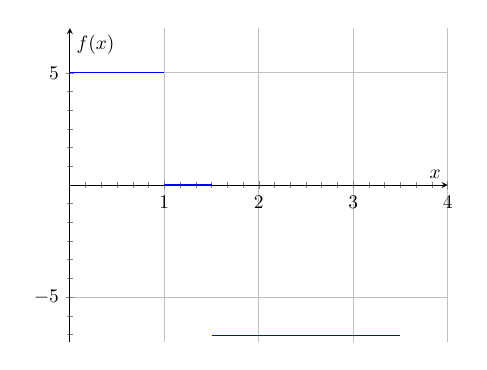
\begin{tikzpicture}[scale=0.7]
    \begin{axis}[
        xlabel={$x$},
        ylabel={$f(x)$},
        axis lines=middle,
        xmin=0, xmax=4,
        ymin=-7, ymax=7,
        samples=100,
            grid, % Activer la grille
            minor tick num=5, % Nombre de divisions mineures entre chaque marqueur majeur
        ]
    
    \addplot[domain=0:1, blue] {5};
      \addplot[domain=1:1.5, blue] {0.02};
      \addplot[domain=1:1.5, blue] {0};
      \addplot[domain=1:1.5, blue] {-0.02};
    \addplot[domain=1.5:3.5, blue] {-6.7};
    \end{axis}
\end{tikzpicture}

 \end{minipage}


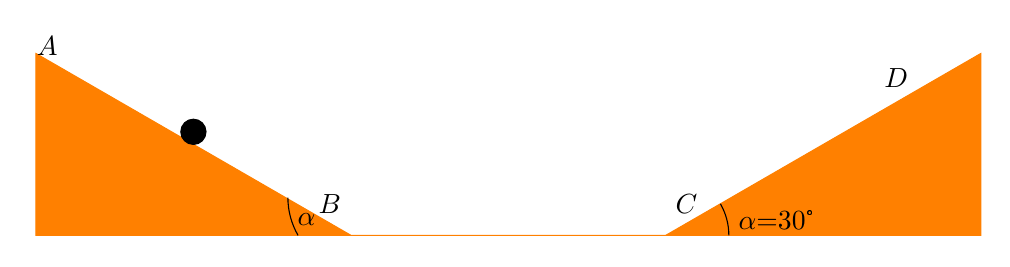
\begin{tikzpicture}[scale=4]
  % Plan incliné
\filldraw[orange](0,0) -- (1,0) -- (1,{1*tan(30)}) -- (0,0) -- cycle;
  % Point
 %   \filldraw (0,0)-- (-1,0) -- (-2,0) -- (-2,{1*tan(30)}) -- (-1,0) -- cycle;
 \filldraw[orange] (0,0)-- (-1,0) -- (-2,0) -- (-2,{1*tan(30)}) -- (-1,0) -- cycle;
  % Point
%   \draw (0,0) -- (-1,0) -- (-1,{-1*tan(30)}) ;
  \filldraw (-1.5,{0.5*tan(30)+0.04}) circle (0.04);
  \node[right] at (0.2,0.05) {$\alpha $=30°};
    \node[right] at (-1.2,0.05) {$\alpha$ };
   \draw (0.2,0) arc (0:30:0.2);
      \draw (-1.2,0.12) arc (0:30:-0.24);*
         \node[left] at (-1.9,0.6) {$A$};
            \node[left] at (-1,0.1) {$B$};
              \node[right] at (0,0.1) {$C$};
                     \node[left] at (0.8,0.5) {$D$};
\end{tikzpicture}




\end{tcolorbox}

\begin{tcolorbox}[sabour,title=EXERCICE 22]

\end{tcolorbox}






\end{document}
